%%%%%%%%%%%%%%%%%%%%%%%%%%%%%%%%%%%%%%%%%
% Beamer Presentation
% LaTeX Template
% Version 1.0 (10/11/12)
%
% This template has been downloaded from:
% http://www.LaTeXTemplates.com
%
% License:
% CC BY-NC-SA 3.0 (http://creativecommons.org/licenses/by-nc-sa/3.0/)
%
%%%%%%%%%%%%%%%%%%%%%%%%%%%%%%%%%%%%%%%%%

%----------------------------------------------------------------------------------------
%	PACKAGES AND THEMES
%----------------------------------------------------------------------------------------

\documentclass[UTF8,aspectratio=169,14pt]{ctexbeamer}

\usepackage{hyperref}
\hypersetup{
	colorlinks=true,
	linkcolor=red,
	anchorcolor=blue,
	citecolor=green
}

\mode<presentation> {
	
	% The Beamer class comes with a number of default slide themes
	% which change the colors and layouts of slides. Below this is a list
	% of all the themes, uncomment each in turn to see what they look like.
	
	%\usetheme{default}
	%\usetheme{AnnArbor}
	%\usetheme{Antibes}
	%\usetheme{Bergen}
	%\usetheme{Berkeley}
	%\usetheme{Berlin}
	%\usetheme{Boadilla}
	%\usetheme{CambridgeUS}
	%\usetheme{Copenhagen}
	%\usetheme{Darmstadt}
	%\usetheme{Dresden}
	%\usetheme{Frankfurt}
	%\usetheme{Goettingen}
	%\usetheme{Hannover}
	%\usetheme{Ilmenau}
	%\usetheme{JuanLesPins}
	%\usetheme{Luebeck}
	\usetheme{Madrid}
	%\usetheme{Malmoe}
	%\usetheme{Marburg}
	%\usetheme{Montpellier}
	%\usetheme{PaloAlto}
	%\usetheme{Pittsburgh}
	%\usetheme{Rochester}
	%\usetheme{Singapore}
	%\usetheme{Szeged}
	%\usetheme{Warsaw}
	
	% As well as themes, the Beamer class has a number of color themes
	% for any slide theme. Uncomment each of these in turn to see how it
	% changes the colors of your current slide theme.
	
	%\usecolortheme{albatross}
	%\usecolortheme{beaver}
	%\usecolortheme{beetle}
	%\usecolortheme{crane}
	%\usecolortheme{dolphin}
	%\usecolortheme{dove}
	%\usecolortheme{fly}
	%\usecolortheme{lily}
	%\usecolortheme{orchid}
	%\usecolortheme{rose}
	%\usecolortheme{seagull}
	%\usecolortheme{seahorse}
	%\usecolortheme{whale}
	%\usecolortheme{wolverine}
	
	%\setbeamertemplate{footline} % To remove the footer line in all slides uncomment this line
	%\setbeamertemplate{footline}[page number] % To replace the footer line in all slides with a simple slide count uncomment this line
	
	%\setbeamertemplate{navigation symbols}{} % To remove the navigation symbols from the bottom of all slides uncomment this line
}

\usepackage{graphicx} % Allows including images
\graphicspath{{./figs/}}
\usepackage{booktabs} % Allows the use of \toprule, \midrule and \bottomrule in tables
\usepackage{longtable}
\usepackage{listings}
\usepackage{xcolor}
\lstset{numbers=left, %设置行号位置
	numberstyle=\tiny, %设置行号大小
	keywordstyle=\color{blue}, %设置关键字颜色
	commentstyle=\color[cmyk]{1,0,1,0}, %设置注释颜色
	frame=single, %设置边框格式
	escapeinside=``, %逃逸字符(1左面的键),用于显示中文
	%breaklines, %自动折行
	extendedchars=false, %解决代码跨页时,章节标题,页眉等汉字不显示的问题
	xleftmargin=2em,xrightmargin=2em, aboveskip=1em, %设置边距
	tabsize=4, %设置tab空格数
	showspaces=false %不显示空格
}
% Fonts
% \usepackage{libertine}
% \setmonofont{Courier}
\setCJKsansfont[ItalicFont=Noto Serif CJK SC Black, BoldFont=Noto Sans CJK SC Black]{Noto Sans CJK SC}


%----------------------------------------------------------------------------------------
%	TITLE PAGE
%----------------------------------------------------------------------------------------

\title[第3讲]{第3讲 进程与调度} % The short title appears at the bottom of every slide, the full title is only on the title page
\subtitle{第五节:实验三:分时多任务系统}
\author{向勇、陈渝、李国良} % Your name
\institute[清华大学] % Your institution as it will appear on the bottom of every slide, may be shorthand to save space
{
清华大学计算机系 \\ % Your institution for the title page
\medskip
\textit{xyong,yuchen,liguoliang@tsinghua.edu.cn} % Your email address
}
\date{\today} % Date, can be changed to a custom date

\begin{document}

\begin{frame}
\titlepage % Print the title page as the first slide
\end{frame}
%----------------------------------------------------------------------------------------
%\begin{frame}
%\frametitle{提纲} % Table of contents slide, comment this block out to remove it
%\tableofcontents % Throughout your presentation, if you choose to use \section{} and \subsection{} commands, these will automatically be printed on this slide as an overview of your presentation
%\end{frame}
%----------------------------------------------------------------------------------------
%	PRESENTATION SLIDES
%----------------------------------------------------------------------------------------

%------------------------------------------------
\section{第五节:教学实验-分时多任务系统}% Sections can be created in order to organize your presentation into discrete blocks, all sections and subsections are automatically printed in the table of contents as an overview of the talk
%------------------------------------------------
\begin{frame}
	\frametitle{系统调用:中断上下文保存与恢复}
    \begin{itemize}
  		\item  TrapContext \href{https://github.com/rcore-os/rCore-Tutorial-v3/blob/ch3-coop/os/src/trap/context.rs\#L4}{结构体}
		\item  \_\_alltraps 的\href{https://github.com/rcore-os/rCore-Tutorial-v3/blob/ch3-coop/os/src/trap/trap.S\#L12}{实现}
		\item 上下文恢复的 \_\_restore 的\href{https://github.com/rcore-os/rCore-Tutorial-v3/blob/ch3-coop/os/src/trap/trap.S\#L40}{实现}
    \end{itemize}	
\end{frame}
%------------------------------------------------
\begin{frame}
	\frametitle{任务切换:任务上下文(Task Context)}
	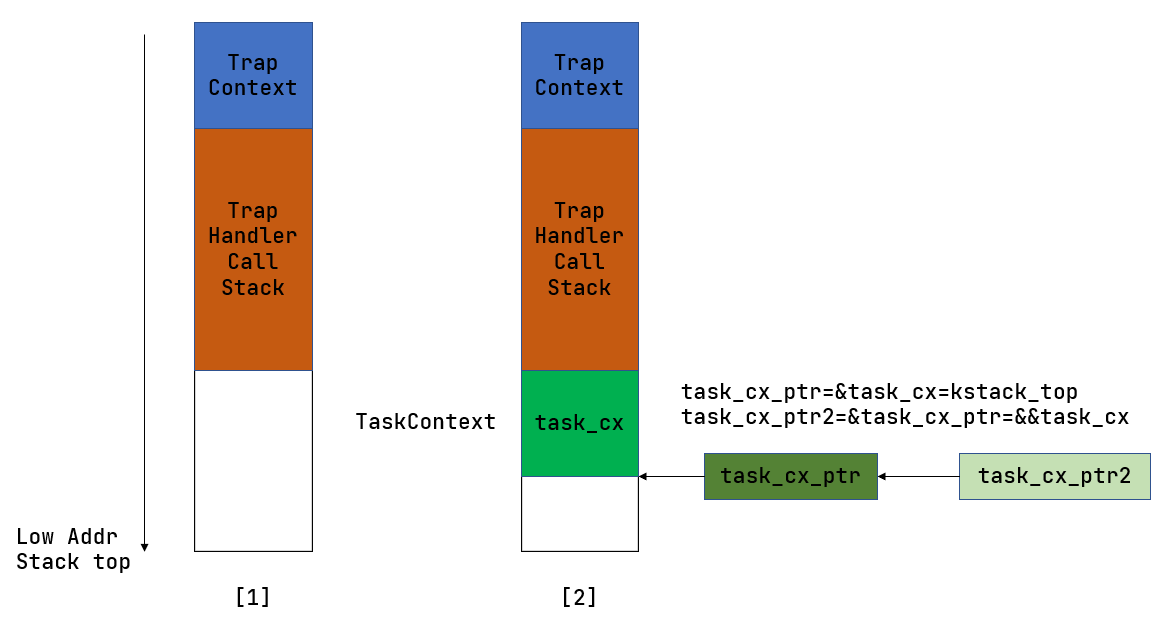
\includegraphics[width=0.7\linewidth]{figs/task_context.png}
	\begin{itemize}
	\item TaskContext \href{https://github.com/rcore-os/rCore-Tutorial-v3/blob/ch3-coop/os/src/task/context.rs\#L2}{数据结构}
	\end{itemize}
\end{frame}
%------------------------------------------------
\begin{frame}
	\frametitle{进程切换过程}
% #### 进程切换过程
% 
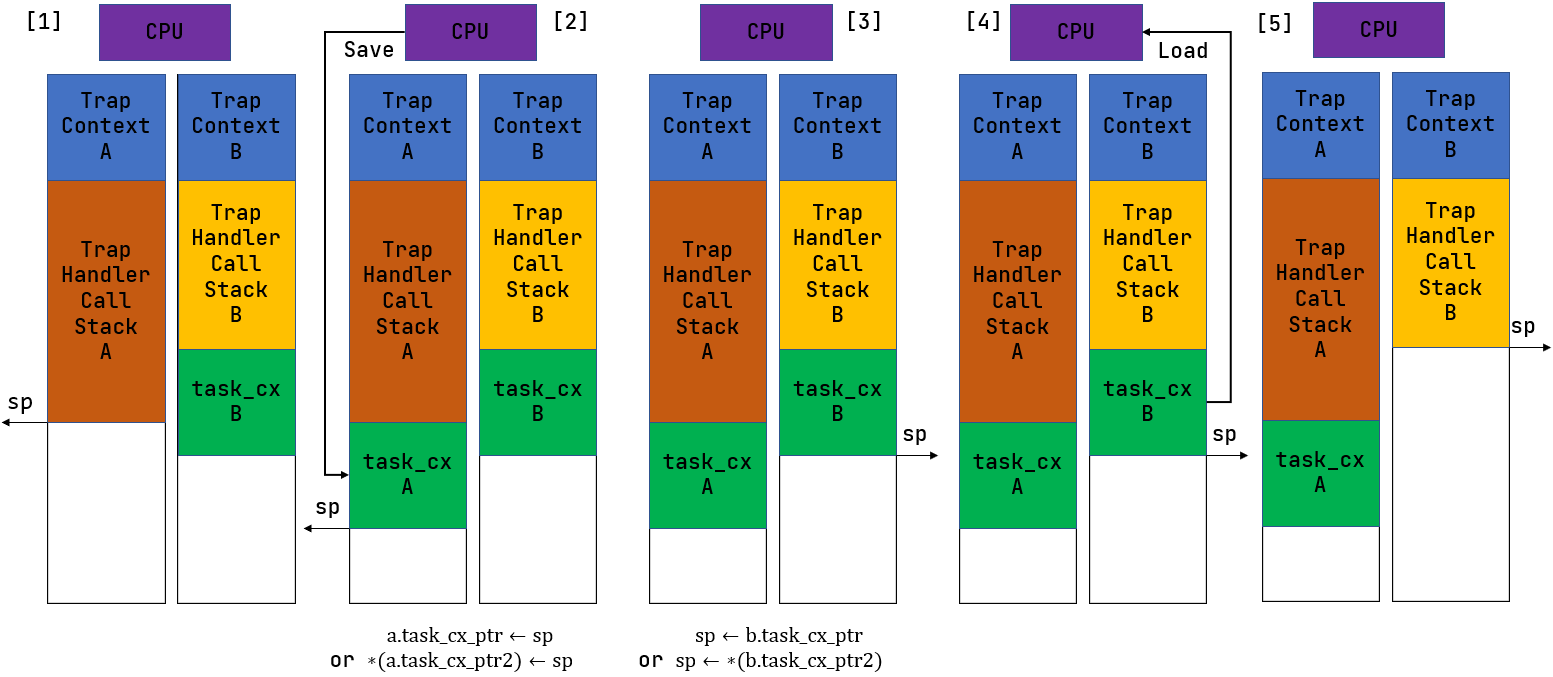
\includegraphics[width=0.9\linewidth]{figs/switch.png}
% 
	\begin{itemize}
		\item \_\_switch 的\href{https://github.com/rcore-os/rCore-Tutorial-v3/blob/ch3-coop/os/src/task/switch.S\#L10}{实现}
	\end{itemize}

\end{frame}
%------------------------------------------------
\begin{frame}
	\frametitle{进程切换的实现}
% #### 进程切换的实现
% 
如何进入用户态第一次执行应用程序?
% 
\begin{itemize}
	\item run\_next\_app \href{https://github.com/rcore-os/rCore-Tutorial-v3/blob/ch2/os/src/batch.rs\#L116}{函数}
	\item app\_init\_context \href{https://github.com/rcore-os/rCore-Tutorial-v3/blob/ch2/os/src/trap/context.rs\#L12}{函数}
\end{itemize}
\end{frame}
%------------------------------------------------
\begin{frame}
	\frametitle{多道批处理系统中的程序加载}
% #### 多道批处理系统中的程序加载
% 
\begin{itemize}
	\item load\_apps \href{https://github.com/rcore-os/rCore-Tutorial-v3/blob/ch3-coop/os/src/loader.rs\#L55}{函数}
\end{itemize}
\end{frame}
%------------------------------------------------
\begin{frame}
	\frametitle{进程管理:任务运行状态}
% #### 进程管理:任务运行状态
% 
简单的进程控制块数据结构和三状态进程模型
% 
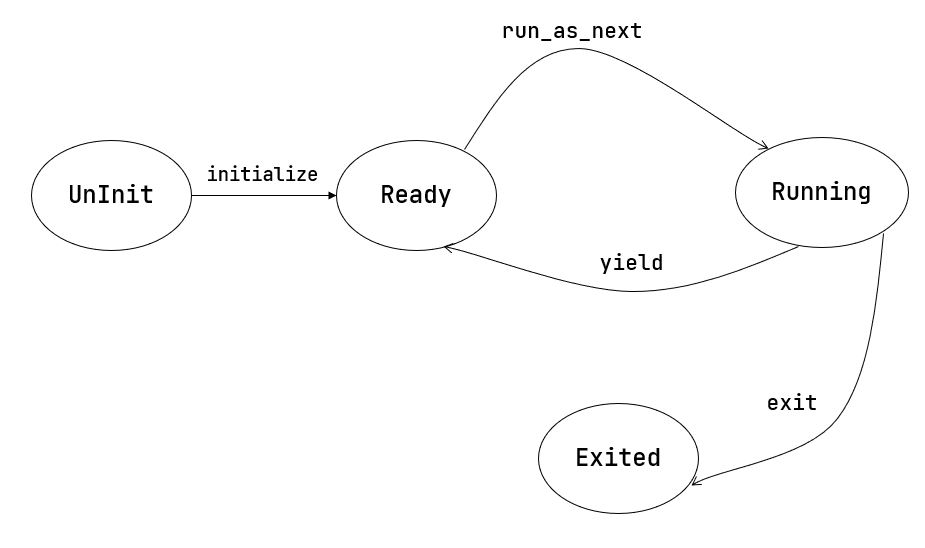
\includegraphics[width=0.6\linewidth]{figs/fsm-coop.png}
% 
\begin{itemize}
	\item  TaskStatus \href{https://github.com/rcore-os/rCore-Tutorial-v3/blob/ch3-coop/os/src/task/task.rs\#L13}{数据结构}
\end{itemize}
\end{frame}
%------------------------------------------------
\begin{frame}
	\frametitle{进程管理:任务控制块}
% #### 进程管理:任务控制块
% 
\begin{itemize}
	\item 任务控制块(Task Control Block): TaskControlBlock  \href{https://github.com/rcore-os/rCore-Tutorial-v3/blob/ch3-coop/os/src/task/task.rs\#L1}{数据结构}

\end{itemize}
\end{frame}
%------------------------------------------------
\begin{frame}
	\frametitle{协作式调度:主动让出CPU}
% #### 协作式调度:主动让出CPU
% 
主动调用sys\_yield来交出 CPU 使用权。

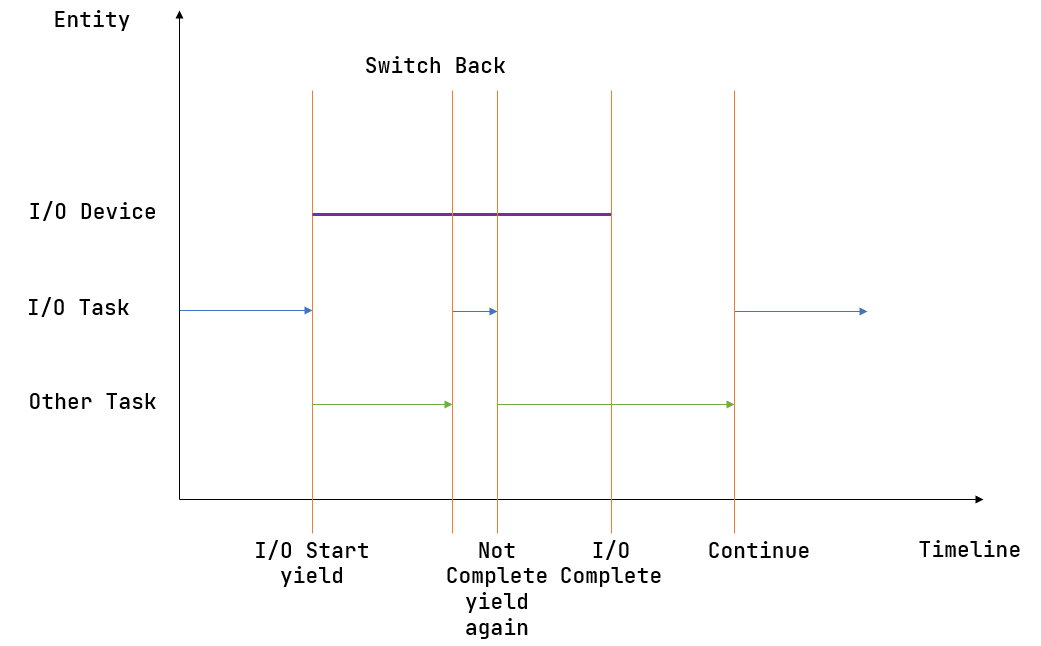
\includegraphics[width=0.7\linewidth]{figs/multiprogramming.png}
\end{frame}
%------------------------------------------------
\begin{frame}
	\frametitle{sys\_yield 和 sys\_exit}
% #### sys_yield 和 sys_exit
% 
\begin{itemize}
	\item sys\_yield \href{https://github.com/rcore-os/rCore-Tutorial-v3/blob/ch3/user/src/syscall.rs\#L27}{系统调用}
	\item  sys\_yield 的\href{https://github.com/rcore-os/rCore-Tutorial-v3/blob/ch3/os/src/syscall/process.rs\#L13}{实现}
	\item  sys\_exit 的\href{https://github.com/rcore-os/rCore-Tutorial-v3/blob/ch3/os/src/syscall/process.rs\#L7}{实现}	
\end{itemize}
\end{frame}
%------------------------------------------------
\begin{frame}
	\frametitle{第一次进入用户态}
% #### 第一次进入用户态
% 
多进程下的第一次进入用户态;
% 
\begin{itemize}
	\item init\_app\_cx 的\href{https://github.com/rcore-os/rCore-Tutorial-v3/blob/ch3/os/src/loader.rs\#L82}{实现}
	\item task::run\_first\_task 的\href{https://github.com/rcore-os/rCore-Tutorial-v3/blob/ch3/os/src/task/mod.rs\#L48}{实现}
	\item  task::run\_next\_task 的\href{https://github.com/rcore-os/rCore-Tutorial-v3/blob/ch3/os/src/task/mod.rs\#L82}{实现}
\end{itemize}
\end{frame}
%------------------------------------------------
\begin{frame}
	\frametitle{第一次进入用户态}
% #### 抢占式调度
% 
\begin{itemize}
	\item timer \href{https://github.com/rcore-os/rCore-Tutorial-v3/blob/ch3/os/src/timer.rs\#L12}{模块}
	\item suspend\_current\_and\_run\_next 的\href{https://github.com/rcore-os/rCore-Tutorial-v3/blob/ch3/os/src/trap/mod.rs\#L53}{引用}和\href{https://github.com/rcore-os/rCore-Tutorial-v3/blob/ch3/os/src/task/mod.rs\#L119}{实现}	
\end{itemize}
\end{frame}
%----------------------------------------------------------------------------------------
\end{document}
